\documentclass[tikz,border=14pt, dvipdfmx]{standalone}
\usepackage{tikz}
\usetikzlibrary{matrix,shapes,decorations.pathreplacing, backgrounds, positioning}

\begin{document}
    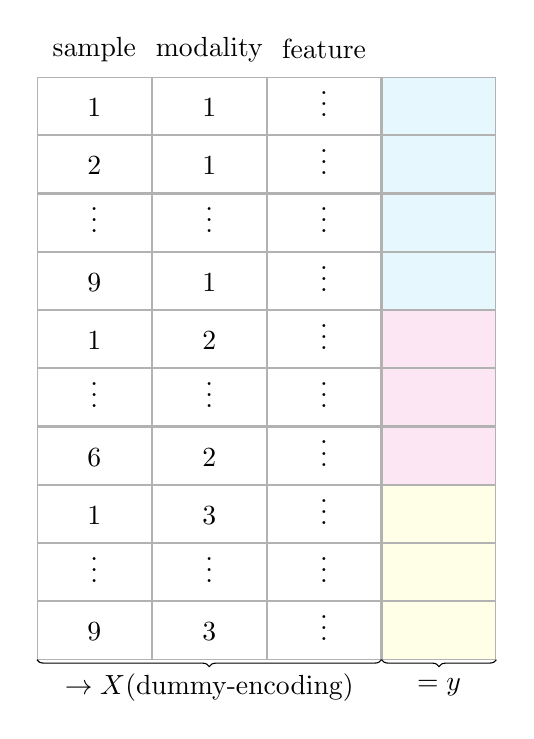
\begin{tikzpicture}[
        %Styles
        Matrix/.style={
            matrix of nodes,
            text height=2.5ex,
            text depth=0.75ex,
            text width=8.0ex,
            align=center,
            column sep=0pt, row sep=0pt,
            nodes={draw=black!30},
            nodes in empty cells,
        }
    ]

%data frame
\matrix[Matrix] at(0,0) (tM){ % Matrix contents  
    1& 1 & \vdots &  \\
    2&  1 & \vdots &  \\
 \vdots& \vdots & \vdots & \\
    9&  1 & \vdots & \\
    1&  2 & \vdots &  \\
    \vdots &  \vdots  & \vdots & \\
    6&   2 & \vdots & \\
    1&  3 & \vdots & \\
    \vdots &  \vdots& \vdots &  \\
    9&  3 & \vdots & \\
};

\node[yshift = 10pt](lab1t) at (tM-1-1.north){sample};
\node[yshift = 10pt](lab2t) at (tM-1-2.north){modality};
\node[yshift = 10pt](lab2t) at (tM-1-3.north){feature};

    \begin{scope}[on background layer]
\foreach \x in {1,...,4}
  \fill [cyan!10] (tM-\x-4.south west) rectangle (tM-\x-4.north east);
\foreach \x in {5,...,7}
\fill [magenta!10] (tM-\x-4.south west) rectangle (tM-\x-4.north east);
\foreach \x in {8,...,10}
\fill [yellow!10] (tM-\x-4.south west) rectangle (tM-\x-4.north east);

\end{scope}

\path[decorate, decoration ={brace, mirror}, draw]
  (tM-10-1.south west) -- (tM-10-3.south east) node[midway, yshift = -10pt]{$\rightarrow X$(dummy-encoding)};

\path[decorate, decoration ={brace, mirror}, draw]
  (tM-10-4.south west) -- (tM-10-4.south east) node[midway, yshift = -10pt]{$=y$};

\end{tikzpicture}
\end{document}